This same sign delepton final state are sensitive to a large range of SUSY processes.
\begin{itemize}
  \item $\chinoonepm\ninotwo$ production when the mass spliting of the $\chinoonepm/\ninotwo$ and $\ninoone$ is small~\cite{Aad:2015eda};
  \item $\chinoonepm\chinoonepm$ pair production from Vector-Boson-Fusion (VBF)~\cite{Aad:2015eda};
  \item $\chinoonepm\ninotwo$ production and decay through $Wh$ final state, where $h\to qq'l\nu$~\cite{Aad:2015jqa}.
  \end{itemize}

The summary of the run 1 results in Fig.~\ref{fig_run1_ew_results}~\cite{susyRun1Summary}.
\begin{figure}[h]
  \centering
  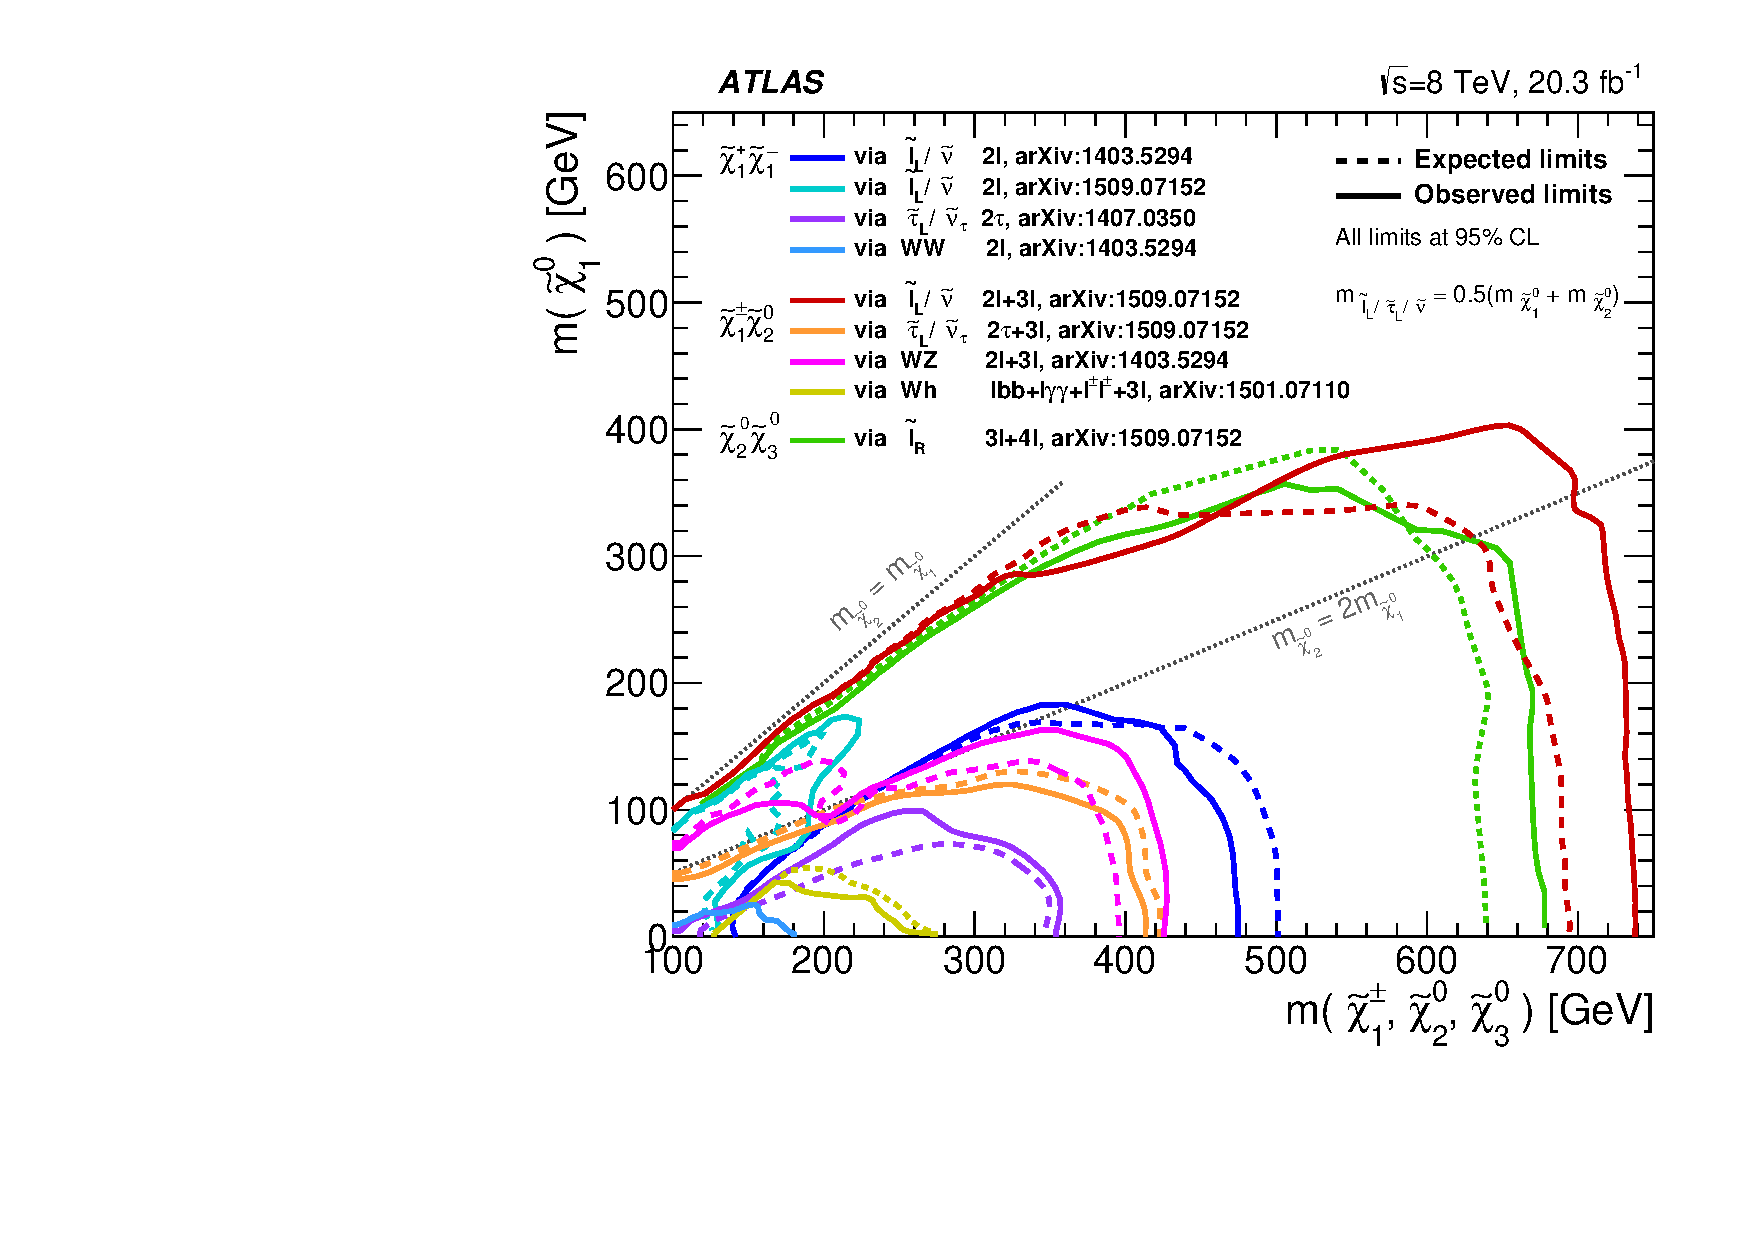
\includegraphics[width=0.7\textwidth]{ATLAS_SUSY_EWSummary}
  \caption{Run 1 summary.}
  \label{fig_run1_ew_results}
\end{figure}

Figure~\ref{fig_run1_soft3l_ss2l} shows the sensitivity of soft/ISR $3l$ and same-sign $2l$ selection. In the left, only $3l$ soft/ISR selection is given separately becasue the contribution from same-sign $2l$ is quite poor (Fig.~\ref{fig_run1_sen1}c). However, as shown in the right figure, the same-sign $2l$ is more sensitive the the case $m_{\susy{l}}=0.95m_{\chinoonepm}+0.5m_{\ninoone}$. The separate limits for the later case is shown in Fig.~\ref{fig_run1_sen2}.
\begin{figure}
  \centering
  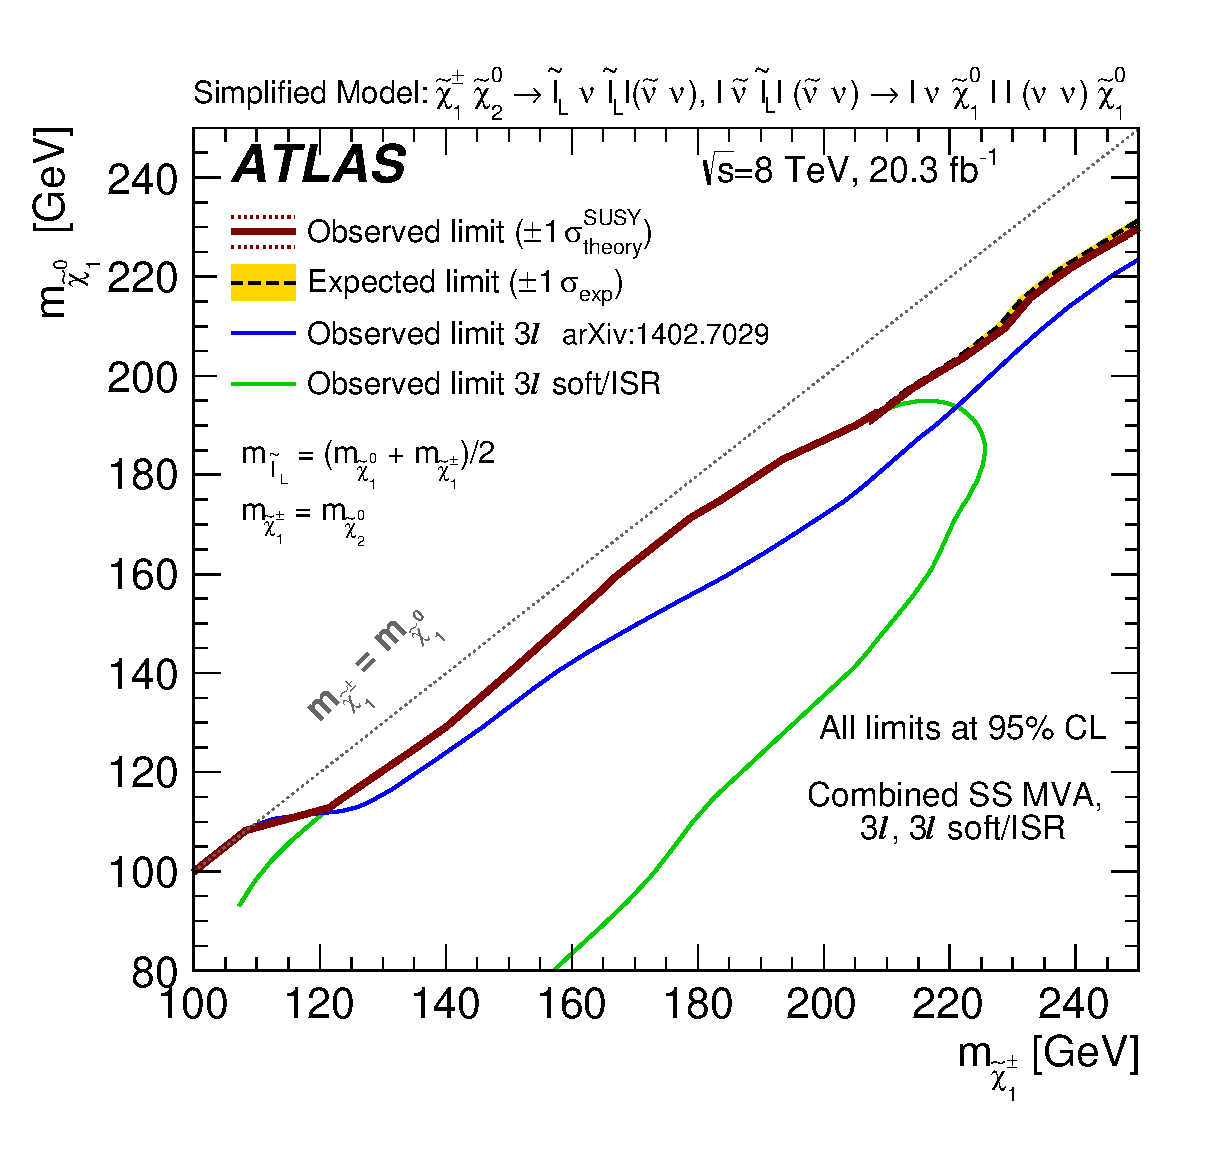
\includegraphics[width=0.49\textwidth]{SUSY_2014_05/fig_17a}
  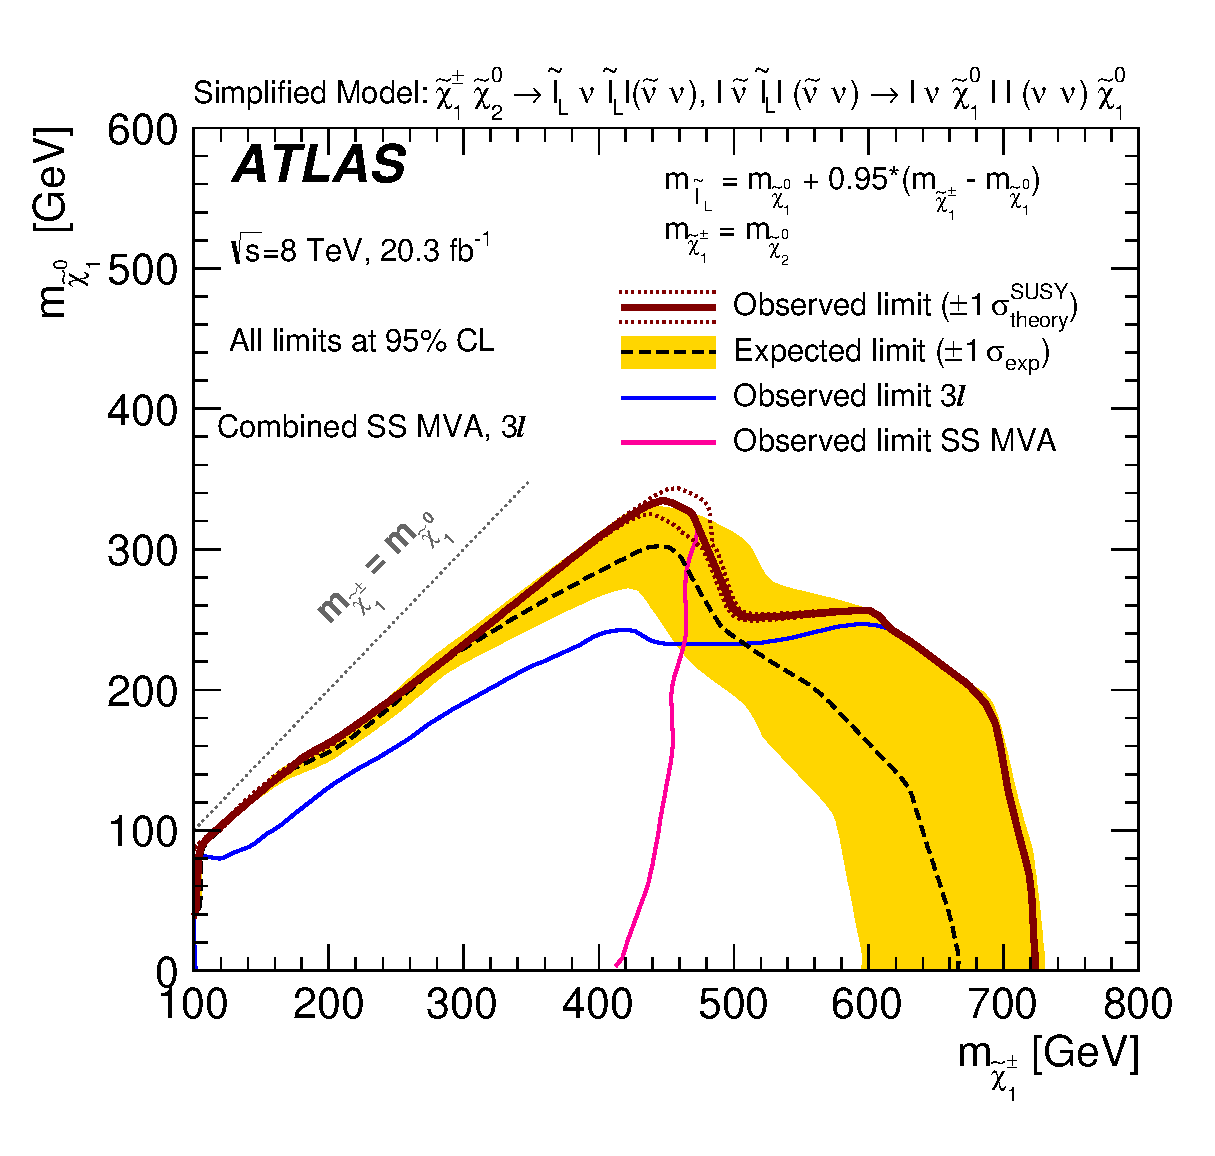
\includegraphics[width=0.49\textwidth]{SUSY_2014_05/fig_17b}
  \caption{The sensitive region of $3l$ soft/ISR selection comparing/combining with the old $3l$ selection (left). The sensitivity of $3l$ soft/ISR selection and same-sign $2l$ is also compared/combined (right). Taken from Ref.~\cite{Aad:2015eda}.}
  \label{fig_run1_soft3l_ss2l}
\end{figure}


% The sensitivity of SS selection is not good in the half mass senario (Fig.~\ref{fig_run1_sen1}), but has strong sensitivity in viarable mass senario (Fig.~\ref{fig_run1_sen2}).

\begin{figure}
  \centering
  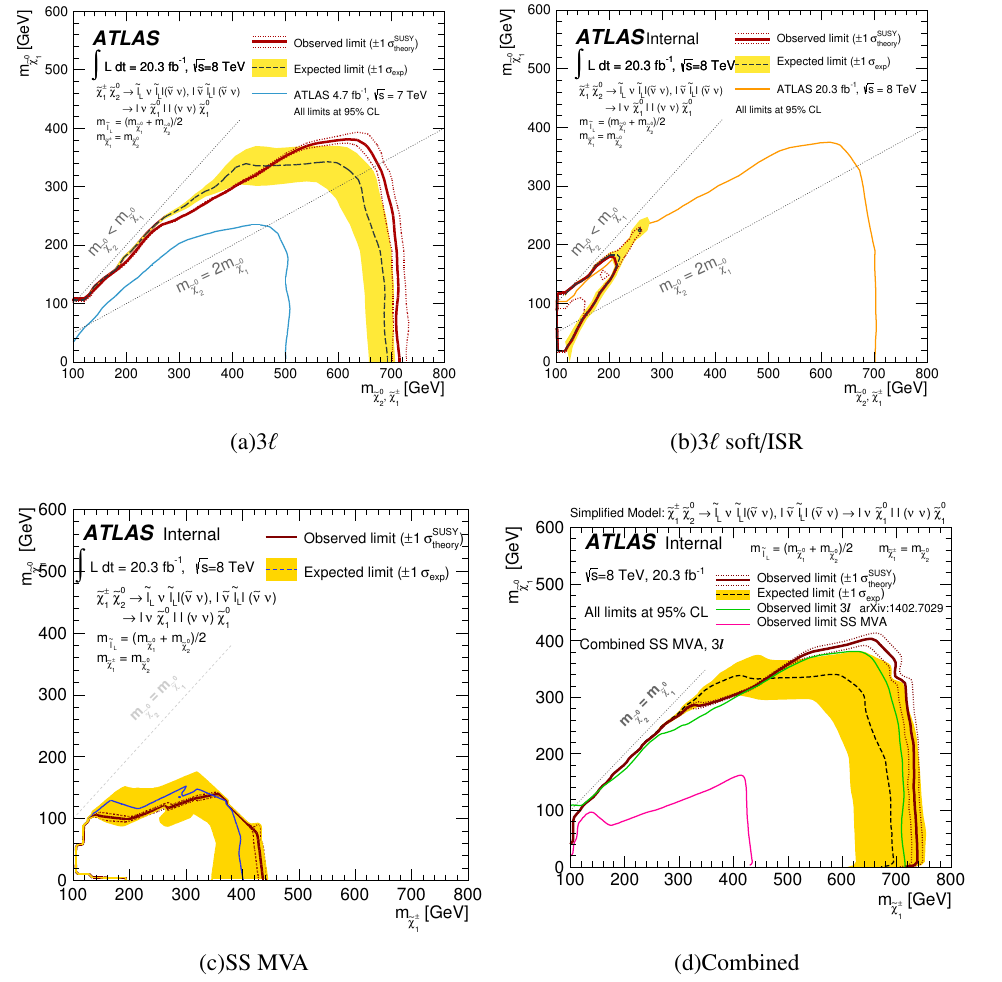
\includegraphics[width=0.9\textwidth]{ATL_COM_PHYS_2015_011/fig_7}
  \caption{Figure 7 of Ref.~\cite{Grout:1981548}}
\label{fig_run1_sen1}
\end{figure}

\begin{figure}
  \centering
  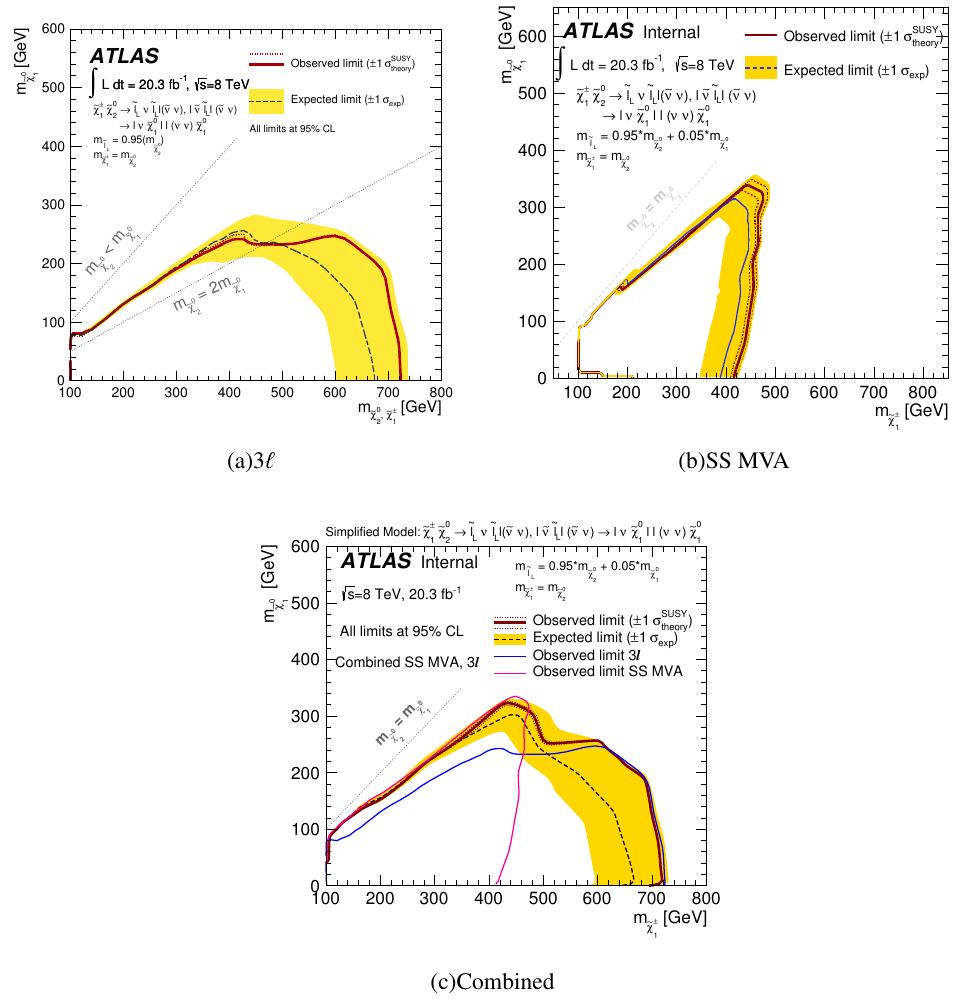
\includegraphics[width=0.9\textwidth]{ATL_COM_PHYS_2015_011/fig_8}
  \caption{Figure 8 of Ref.~\cite{Grout:1981548}}
\label{fig_run1_sen2}
\end{figure}


% \begin{figure}
%   \centering
%   \includegraphics[width=0.49\textwidth]{SUSY_2014_05/fig_19a}
%   \includegraphics[width=0.49\textwidth]{SUSY_2014_05/fig_19b}
% \end{figure}


The cross section of the signal is shown in Fig.~\ref{fig_sig_xsec}.
\begin{figure}
  \centering
  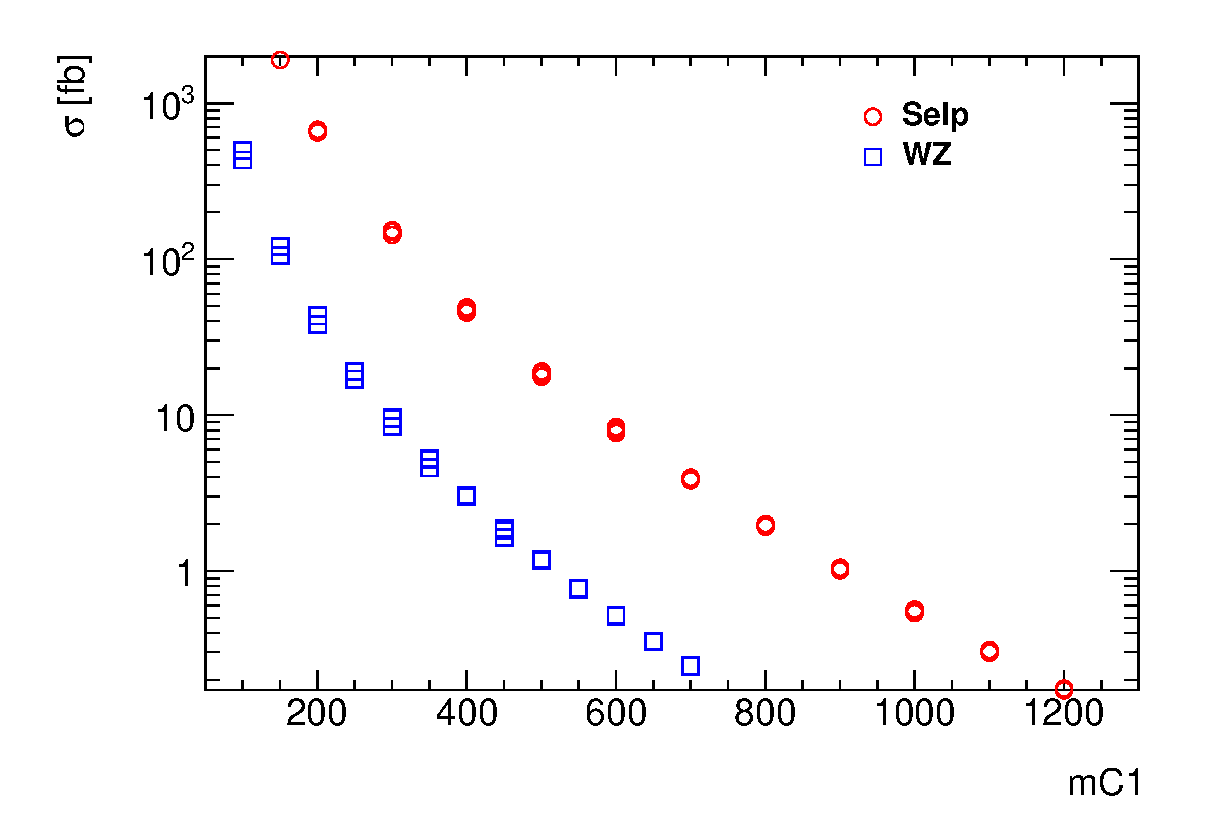
\includegraphics[width=0.49\textwidth]{sig_xSec}
  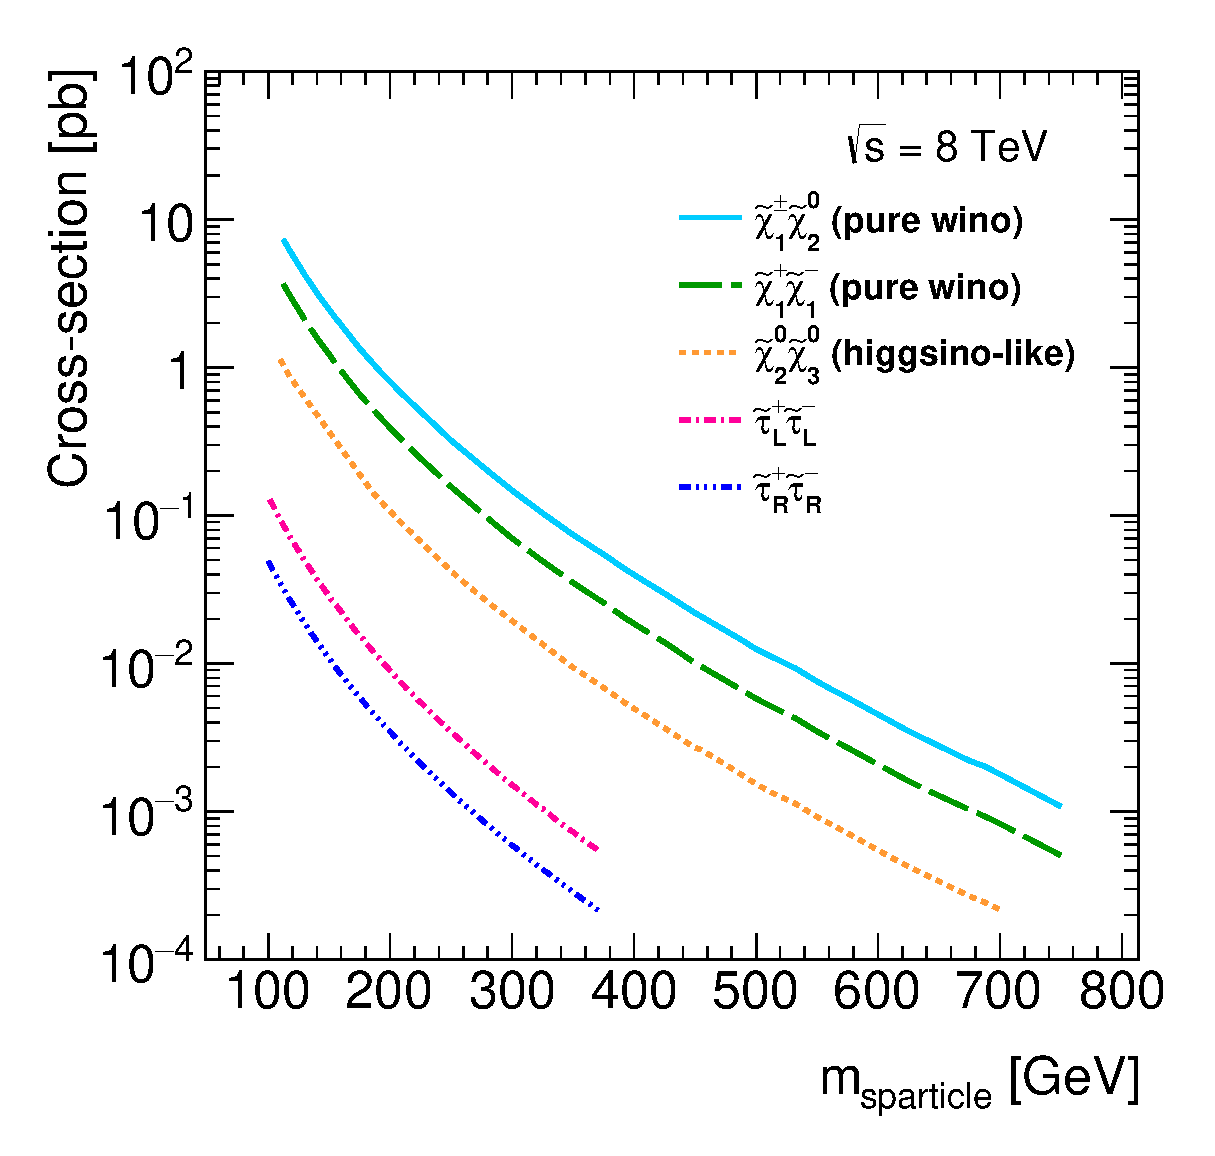
\includegraphics[width=0.49\textwidth]{SUSY_2014_05/fig_01}
  \caption{Cross section of $\chinoonepm\ninotwo$ production in $13\TeV$ and $8\TeV$ (from~\cite{Aad:2015eda}).}
  \label{fig_sig_xsec}
\end{figure}
